\chapter{Experiments and Results} % Main chapter title

\label{Chapter7} % Change X to a consecutive number; for referencing this chapter elsewhere, use \ref{ChapterX}

\section{Speedup}

% spm speedup
% infinite spm
% pinning

We show the estimated performance benefits of our optimal strategy in figure
\ref{fig:speedup}. The figure shows the speedup as a percentage of the baseline
performance. We show that we can more than a 1.5x improvement in performance
using our spm management strategy for even the smallest spm size we test on. It
also shows that we show that we reach close to our roofline performance of a
infinite scratchpad even for our base architecture configuration of a 32kb size
per scratchpad for some models.

\begin{figure}[thb!]
\centering
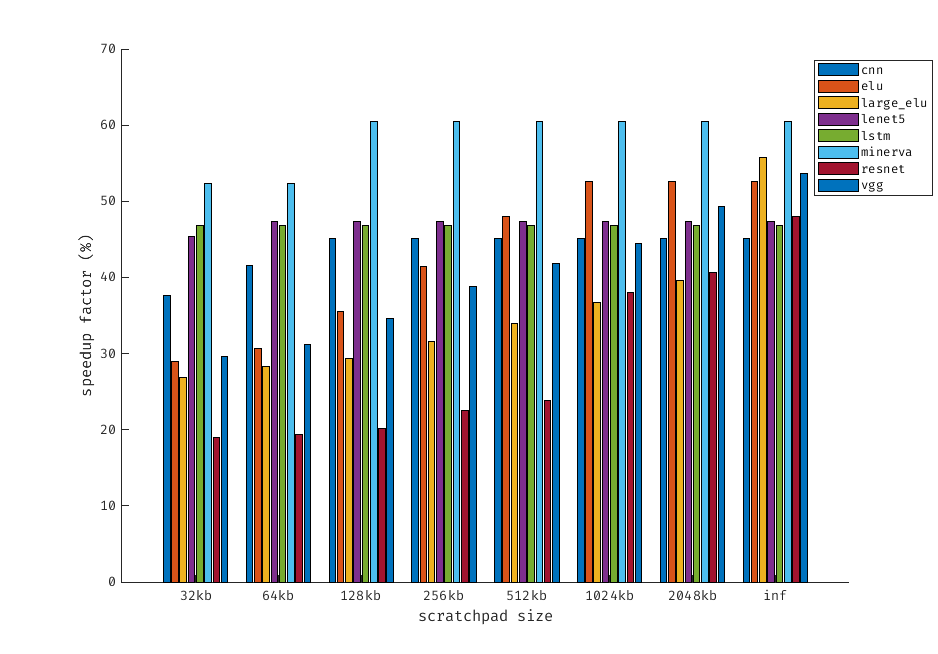
\includegraphics[scale=0.7]{Figures/speedup_factor.png}
\decoRule
\caption[Speedup Results]{Estimated speedup for varying scratchpad sizes and models using the optimal pinning strategy}
\label{fig:speedup}
\end{figure}

% table with average speedup for each of the sizes and overall speedup %s
The table \ref{tab:memory_bound} shows how memory bound each model architecture
is, i.e the fraction of total cycles spent on DMA transfers, and the possible
speedup if one were to eliminate DMA transfers in totality. Next to those
metrics, the possible speedup gained if we applied our strategy to an infinite
capacity SPM is shown next to the average gained speed up for all SPM sizes
tested on. On average we achieve at least a 1.41x speedup across all models.
At a minimum 1.19x speedup can be obtained for the worst case and 1.60x speedup
for the best case.

\begin{table}[]
	\begin{tabular}{|l|l|l|l|l|}
		\hline
		Model     & Memory Boundness & Theoretical Speedup & Inf SPM Speedup & Average Speedup\\ \hline
		CNN       & 39.83\%          & 66.20\%             & 45.16\%              & 41.81\%        \\ \hline
		Lenet5    & 40.79\%          & 68.89\%             & 47.30\%              & 42.91\%        \\ \hline
		Lstm      & 42.27\%          & 73.21\%             & 47.76\%              & 42.93\%        \\ \hline
		Minerva   & 47.65\%          & 91.04\%             & 60.46\%              & 43.10\%        \\ \hline
		Elu       & 43.81\%          & 77.96\%             & 52.66\%              & 42.08\%        \\ \hline
		Large-Elu & 45.21\%          & 82.51\%             & 55.81\%              & 42.55\%        \\ \hline
		Resnet    & 41.50\%          & 70.95\%             & 48.01\%              & 43.10\%        \\ \hline
		VGG       & 44.12\%          & 78.95\%             & 53.65\%              & 43.71\%        \\ \hline
	\end{tabular}
	\caption[Comparison of Speedup Acheived and Upper Bound Speedup]{Memory Boundness, upper bound of speedup if no DMA transfers were needed at all, the speedup possible from an SPM with infinite capacity, the average
	speedup for all capacities tested on for each model}
	\label{tab:memory_bound}
\end{table}

Figure \ref{fig:max} shows for each SPM capacity tested, how much of the
maximum achieved speedup given an infinite sized SPM our pinning strategy
obtained. It can be seen that DNN workloads with sequential operator scheduling
such as Lenet5, Minerva, and Elu quickly converge to the maximum possible
speedup given an infinite SPM since every output simply gets pinned for
immediate reuse until there there is a capacity limit. At the worst case for Resent
on the 32Kb SPM size, we obtain a 39.5\% of the max achievable speedup and 100\% for
LSTM, Minerva, Lenet5, and CNN for SPM sizes of at least 128Kb.

\begin{figure}[!htb]
\centering
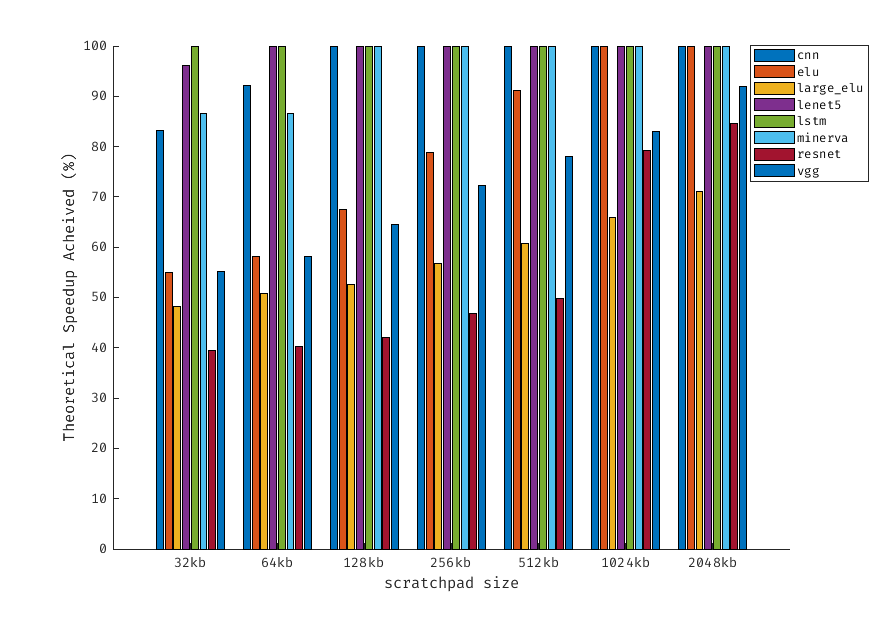
\includegraphics[scale=0.7]{Figures/max_acheived.png}
\decoRule
\caption[Percentage of Max Speedup Obtained]{How much of the theoretical speedup from an infinite sized SPM was achieved in (\%) for each SPM capacity}
\label{fig:max}
\end{figure}

% SPM reduction factor
% Infinite SPm
% pinning

\section{Reduction of DMA Transfers}

Figure \ref{fig:Reduction} shows a plot of how much of the total necessary
transfers were avoided through our pinning strategy. It is noted that the
infinite SPM still does not meet 100\% data transfers saved since inputs and
weights must still be initially loaded into the SPM.

Similar to the speedup increase as scratchpad size increases, we see a linear
correlation of increased scratchpad size and the total data transfers saved.
For the same models where the maximum efficiency was obtained, we see that the
savings in DMA costs are also close to the maximum achievable savings. Figure
\ref{fig:Saved} illustrates this by showing the percentage of total DMA
transfers incurred versus the minimum achievable DMA transfers incurred by an
infinite capacity SPM for each SPM size tested.

It appears that regardless of how sequential operators may seem to be connected
in a graph, the scheduled ordering of the operators matters much much more in
terms of how reusable the outputs become. Clearly, even though LSTM seems much
more complex of an architecture with many diverging paths, our pinning strategy
still achieves its maximum possible speedup before sequential models such as
Minerva and obtains a higher overall speedup to VGG.

\begin{figure}[thb!]
\centering
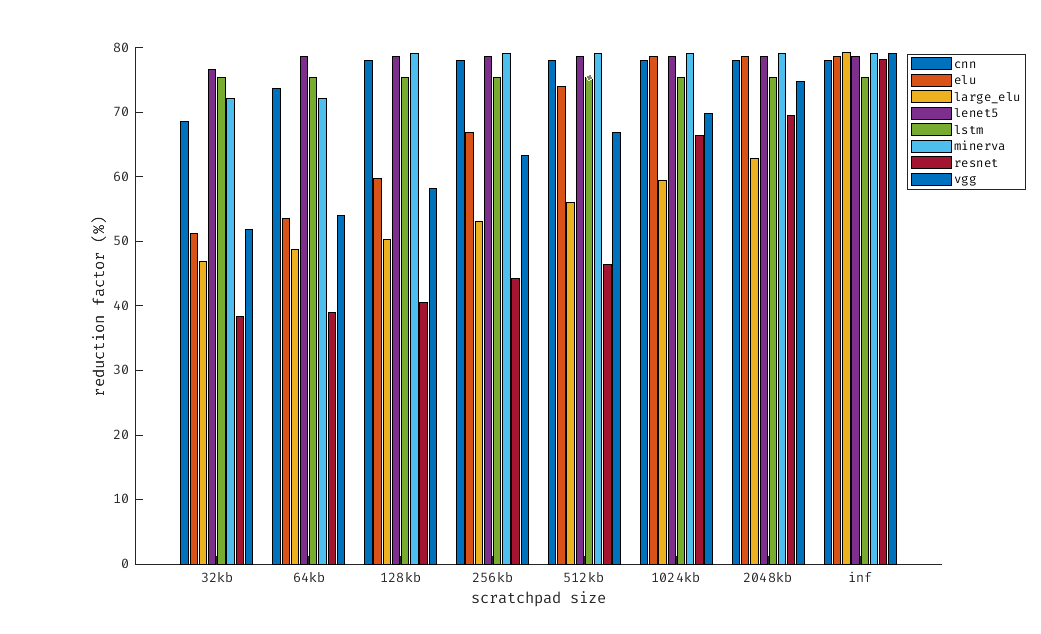
\includegraphics[scale=0.5]{Figures/reduction_factor.png}
\decoRule
\caption[Results of Data Transfer Costs Saved]{Estimated \% of data transfers saved for varying scratchpad sizes and models using the optimal pinning strategy}
\label{fig:Reduction}
\end{figure}


\begin{figure}[thb!]
\centering
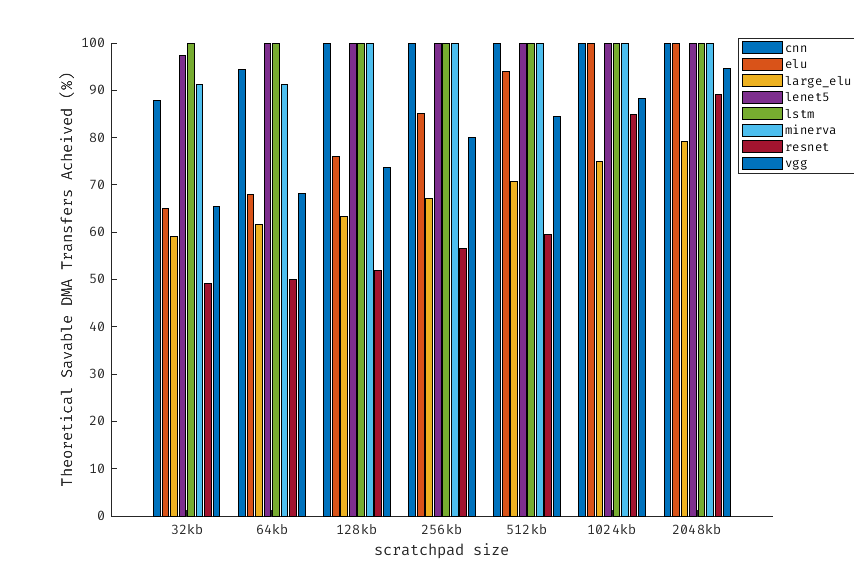
\includegraphics[scale=0.7]{Figures/max_saved.png}
\decoRule
\caption[Percentage of Max Data Transfers Saved]{Percentage of total DMA transfers incurred versus the minimum achievable DMA transfers incurred by an infinite capacity SPM for each SPM size tested}
\label{fig:Saved}
\end{figure}

\section{Discussion of Results}
Given our results, we conclude that a pinning strategy on a graph with no tiling and capped tensor sized can achieve at least 40\% of the theoretical maximum
speedup and DMA cost savings and for some cases the maximum. We note that, although the maximum capped tensor size was scaled to be the size of the SPM for each
experiment, we still see a linear increase in speedup and DMA cost savings as the SPM capacity increases. In some cases, the size of the tensor does not matter
due to the workload characteristics and operator schedule.

The results are difficult to compare against different hardware arhictures,
simulators, models, and number of scratchpads. Still, we compare OnSRAM results
to ours. OnSRAM tests on a 2MB SPM DLA so we will be comparing our 1024KB
scratchpad results as the closest comparison in terms of total SPM capacity.
OnSRAM-static obtains an average of 50\% increase in performance relative to
their baseline SPM management strategy and achieves 90\% of the ideal infinite
SPM \cite{onsram}. However, out of the 13 DNN workloads evaluated on, only 5 of
those models reach over a 50\% increase while the rest remain under a 20-30\%
speedup. In comparison we achieve a minimum of a 40\% speedup across all
workloads from our baseline 32Kb configuration and a minimum of 65\% of ideal
speedup obtained for the 1024Kb configuration. The models that both our work
and OnSRAM has evaluated include: VGG, Lenet, and Resnet. For all three cases,
both OnSRAM-Static and our strategy gains most of the of ideal performance
possible.  Overall, it seems as though the greedy strategy achieves close to
the optimal, and in some cases the optimal, level of performance possible. This
may mean for the single scratchpad case, the overhead required for an ILP
solver may not be necessary.

% table with average reduction and medium reduction for each of the sizes and overall reduction %s

% disucssion around sequential DNNS: VGG, CNN, Minerva
% discussion around non-sequential

% upper bound of no transfers
% upper bound of infinite SPM

% degree of SPM pinning: Compute bound vs memoyr bound fraction of tesnors pinned
% average operation reuse for pinned tenosors %s
